%!TEX root = ../dissertation.tex
\chapter{Related Work}
Programming language has been developed for about 60 years. There are a lot of popular and mature designs have been introduced into the computer language's world. Nowadays, C and Java are the most popular system level and static type programming language. Python will be a good representative for the scripting and dynamic type language. In this chapter, we will discuss the modern programming languages. For the machine level, we will discuss the MIPS, a reduced assembly language. Last but not least, we will take a look of LLVM and Java virtual machine

\section{Python, Java \& C, Modern Programming Languages}
C is a general-purpose, imperative computer programming language, supporting structured programming, lexical variable scope and recursion, while a static type system prevents many unintended operations. By design, C provides constructs that map efficiently to typical machine instructions, and therefore it has found lasting use in applications that had formerly been coded in assembly language, including operating systems, as well as various application software for computers ranging from supercomputers to embedded systems. \\
In current high level programming language world, C is always considered as a low level programming language since it can manipulate the memory directly. Another example is the Python and Java, although they are able to perform some low level instruction, they are virtual machine based and the Just In Time compiler translates the virtual machine instruction to the machine instruction on fly. \\
Unlike other two languages, the Python programming language is dynamic type and every thing in python is an object. The low level representation of Python variable is the \texttt{PyObject} struct in C. The run time type is stored in the \texttt{PyObject} and the Python virtual machine checks the correctness of the type for every assignment.

\section{MIPS, A reduced Assembly Language}
MIPS is a reduced instruction set computer (RISC) instruction set architecture (ISA) developed by MIPS Technologies. The MIPS code is a 3 address codes and there are 3 operands in one instruction at the same time. An example MIPS code is the \texttt{add} instruction: \texttt{add \$0 \$0 \$1}. The first operand in MIPS is the target operand which stores the result. The second and third operands are the operand of the operation. This instruction style allows the instruction set to be in SSA form, in which case, every variable in the code is assigned only once.


\section{LLVM's bit code, Static Single Assignment Form}
The LLVM Project is a collection of modular and reusable compiler and toolchain technologies. LLVM can be used as a compiler framework, where you provide the "front end" (parser and lexer) and the "back end" (code that converts LLVM's representation to actual machine code). In the Clang compiler, which is a front end and a compiler driver of LLVM, it translates the C code to LLVM bit code, or LLVM IR. \\
\begin{figure}[h]
\centering
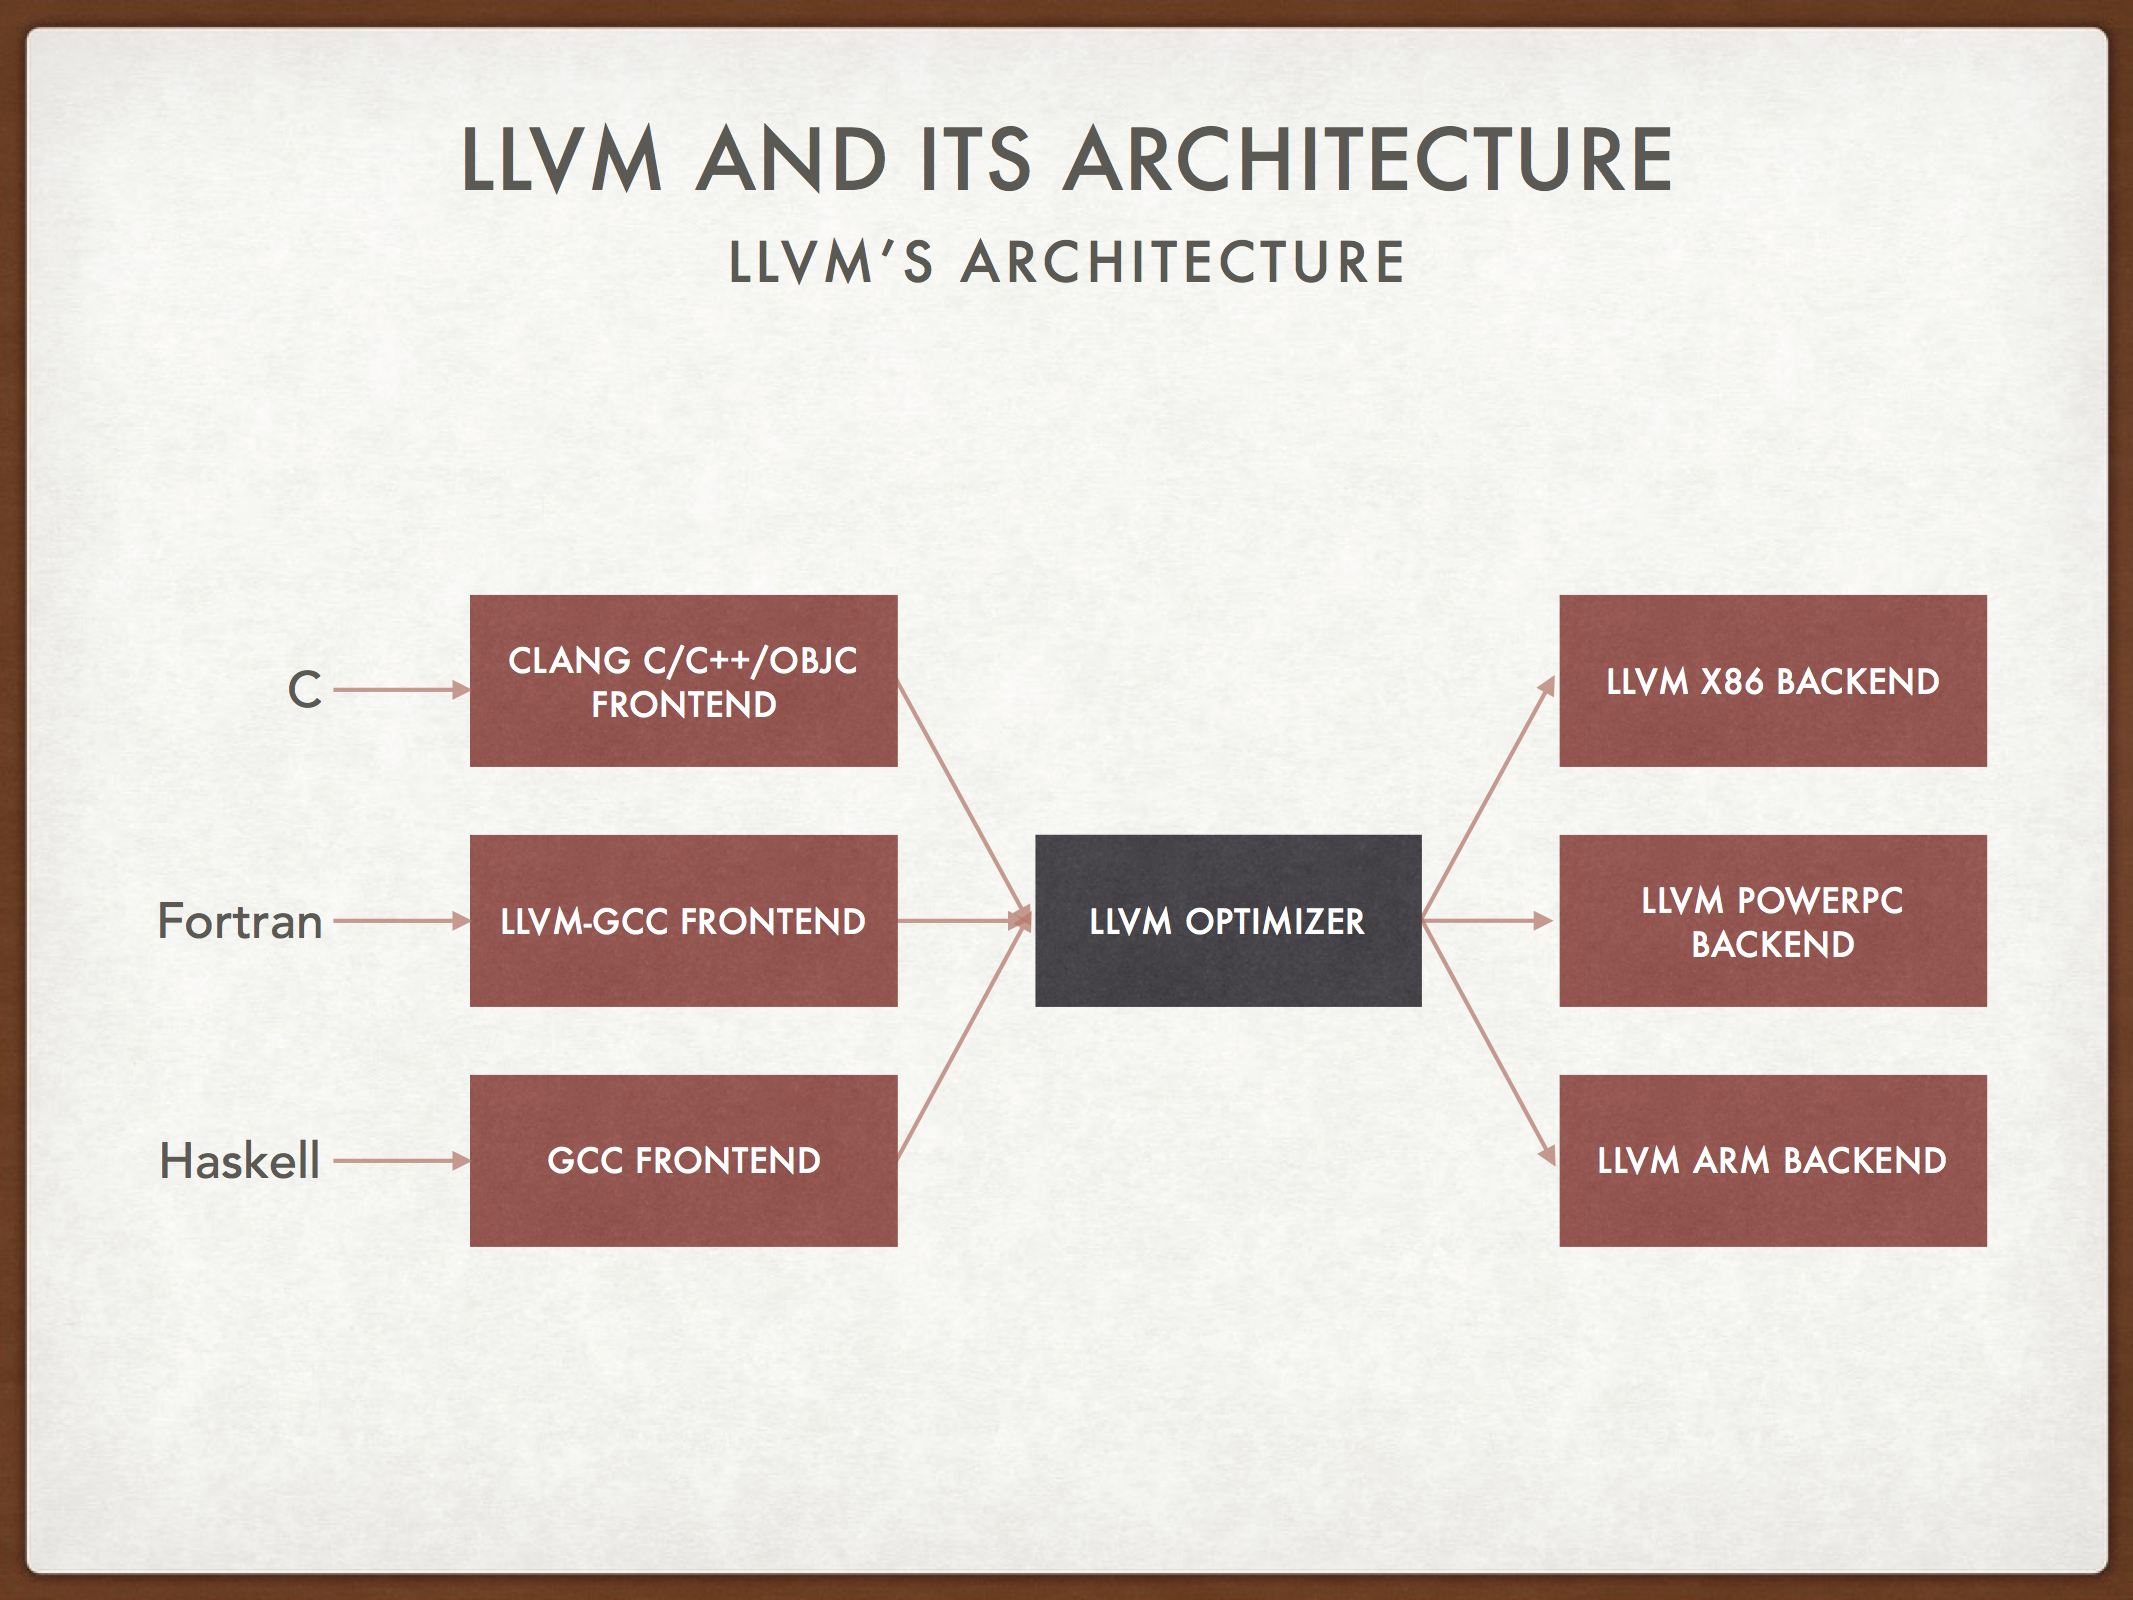
\includegraphics[width=10cm]{LLVM}
\end{figure}
Developed by Ron Cytron, Jeanne Ferrante, Barry K. Rosen, Mark N. Wegman, and F. Kenneth Zadeck, researchers at IBM in the 1980s, static single assignment form (often abbreviated as SSA form or simply SSA) is a property of an intermediate representation (IR), which requires that each variable is assigned exactly once, and every variable is defined before it is used. Existing variables in the original IR are split into versions, new variables typically indicated by the original name with a subscript in textbooks, so that every definition gets its own version. In SSA form, use-def chains are explicit and each contains a single element. \\
LLVM IR is a Static Single Assignment (SSA) based representation that provides type safety, low-level operations, flexibility, and the capability of representing ‘all’ high-level languages cleanly. The LLVM optimizer will then optimize the code of the LLVM IR and finally the backend generator will generate the machine code for every instructions in LLVM IR. \\


\section{Java \& Python, Instruction over Virtual Machine}
Aliquam feugiat turpis at metus ultrices, quis elementum justo gravida. Suspendisse mi lacus, aliquet at nisi at, varius aliquet sem. Donec venenatis, arcu eget feugiat suscipit, eros sem maximus ante, quis varius sem metus non nulla. Mauris euismod elit mi, ac viverra magna cursus a. Morbi id elementum nisi, ac varius turpis. Etiam vehicula, leo non faucibus aliquam, libero leo pulvinar ipsum, id hendrerit justo sem maximus lectus. Vivamus semper elit ut metus iaculis, pellentesque convallis urna vulputate. Pellentesque gravida porttitor dignissim. Sed sit amet elit nulla. Sed consequat faucibus purus, in gravida arcu tristique ac. Nullam et pellentesque purus. Nulla facilisi. Pellentesque finibus dolor at sem ornare, et vulputate mi consequat. Donec a leo at lorem convallis mattis.

Pellentesque pharetra ultrices ante, id efficitur mi venenatis quis. Curabitur eget faucibus lectus, ut posuere diam. Nulla ornare vulputate ante, in euismod tellus cursus quis. Sed rutrum sem elit, eu dictum quam tempor ac. Etiam porttitor orci ut tellus euismod ornare. Vivamus eu sollicitudin quam, ac convallis est. Nulla eros magna, mattis ac dignissim ut, mattis id orci. Curabitur non orci sit amet turpis ullamcorper vehicula. Praesent mattis quam at nunc egestas tempus. Fusce blandit massa nec massa dignissim, eget aliquam leo aliquam. Sed ut massa vel lacus faucibus rutrum. Donec scelerisque efficitur semper. Curabitur ut erat et dui pellentesque aliquet rutrum in erat. Praesent id odio nulla. Nulla sollicitudin nisl in est molestie molestie. Morbi euismod sagittis cursus.
